\documentclass[tikz,convert={density=600,outext=.jpg},border=5pt]{standalone}
%\documentclass[tikz, border=5pt]{standalone}

\usepackage[utf8]{inputenc} % utf8 encoding
\usepackage[english]{babel}
\usepackage[T1]{fontenc} % use T1 fonts
\usepackage{amsmath} % nice math symbols
     

\usepackage{tikz}
\usetikzlibrary{shapes, arrows,calc,decorations.markings}

\begin{document}
	
	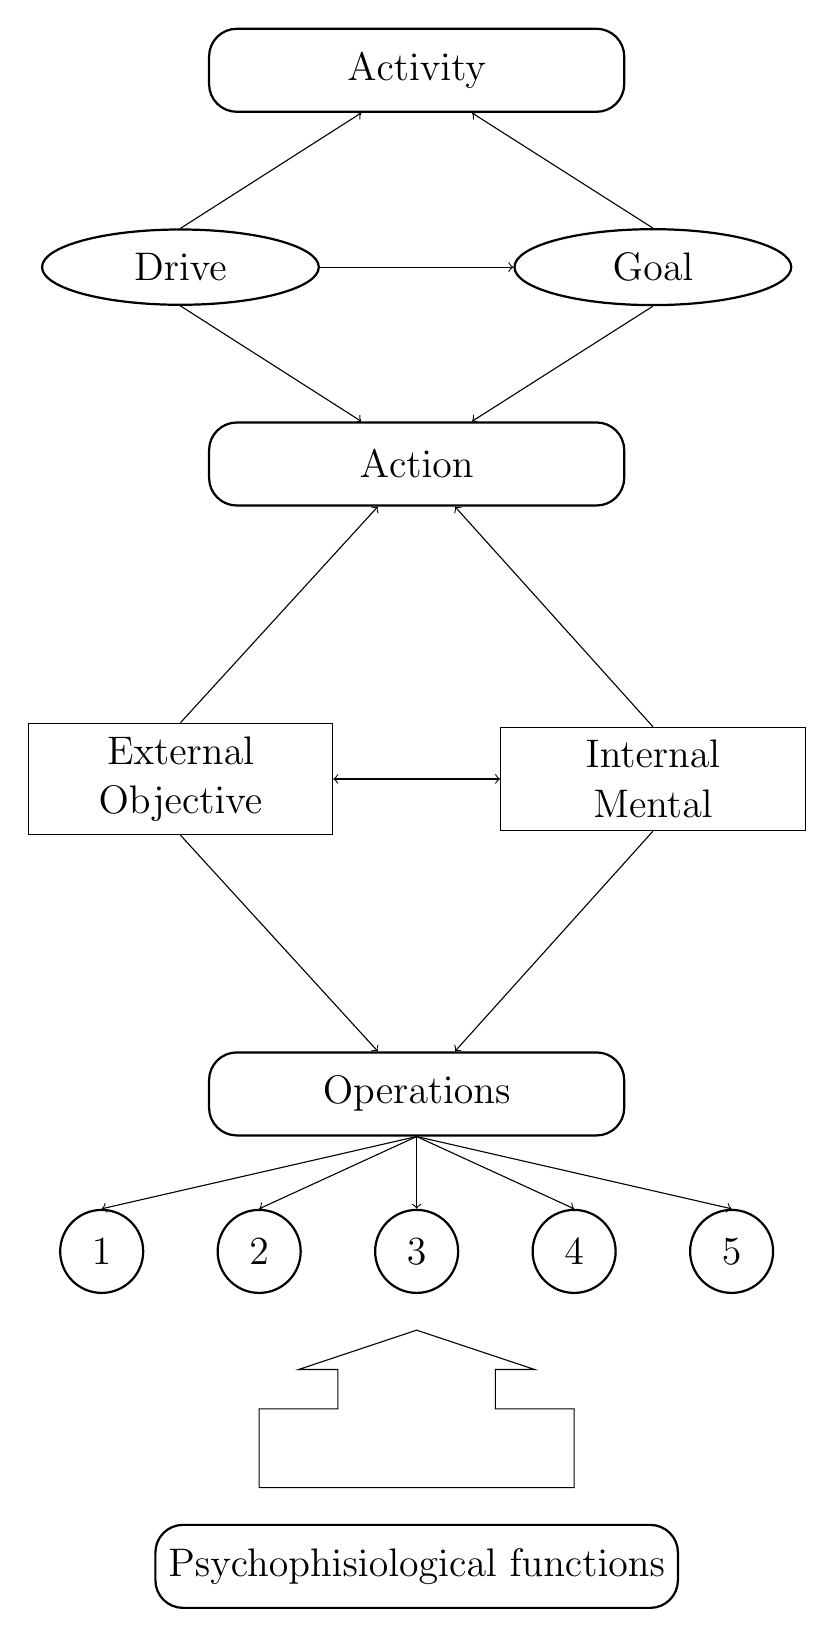
\begin{tikzpicture}
		\Large
		\tikzstyle{round_block} = [draw, thick, rectangle, rounded corners=10, minimum height = 30, minimum width = 150,align = center];
		\tikzstyle{cir_block} =[draw, thick, circle, minimum width = 30, minimum height = 30,align = center];
		\tikzstyle{ell_block} =[draw, thick, ellipse, minimum width = 100, minimum height = 20, align = center];
		\tikzstyle{rect_block} = [draw, rectangle, minimum width = 110, minimum height = 30, align=center]

		\node[round_block] (act) at (0,0) {Activity};
		
		\node[ell_block] (mot) at (-3,-2.5) {Drive};
		\node[ell_block] (goal) at (3,-2.5) {Goal};
		
		\node[round_block] (pred) at (0,-5) {Action};
		
		\node[rect_block] (exter) at (-3,-9) {External\\Objective};
		\node[rect_block] (inter) at (3,-9) {Internal\\Mental};
		
		\node[round_block] (oper) at (0,-13) {Operations};
		
		\foreach \i in {1,...,5}{%
			\node[cir_block] (thisNode) at ($(-6,-15)+(2*\i,0)$) {\i};
			\draw[<-] (thisNode.north) -- (oper.south);
		}
		
		\node[round_block] (func) at (0,-19) {Psychophisiological functions};
		
		\draw[->] (mot.north) -- ([xshift=-20]act.south);
		\draw[->] (goal.north) -- ([xshift=20]act.south);
		\draw[->] (mot.east) -- (goal.west);
		\draw[->] (mot.south) -- ([xshift=-20]pred.north);
		\draw[->] (goal.south) -- ([xshift=20]pred.north);
				
				
		\draw[->] (exter.north) -- (pred);
		\draw[->] (inter.north) -- (pred);
		\draw[->] (exter.south) -- (oper);
		\draw[->] (inter.south) -- (oper);
		
		\draw[<->] (exter) -- (inter);
		
		\draw (-2,-18) -- (-2,-17) -- (-1,-17) -- (-1,-16.5) -- (-1.5,-16.5) -- (0,-16)
		-- (1.5,-16.5) -- (1,-16.5) -- (1,-17) -- (2,-17) -- (2,-18) -- (-2,-18);
	\end{tikzpicture}

\end{document}